%%%%%%%%%%%%%%%%%%%%%%%%%%%%%%%%%%%%%%%%%%%%%%%%%%%%%%%%
%                IAML 2020 Assignment 2                %
%                                                      %
%                                                      %
% Authors: Hiroshi Shimodaira and JinHong Lu           %
% Based on: Assignment 1 by Oisin Mac Aodha, and       %
%          Octave Mariotti                             %
% Using template from: Michael P. J. Camilleri and     %
% Traiko Dinev.                                        %
%                                                      %
% Based on the Cleese Assignment Template for Students %
% from http://www.LaTeXTemplates.com.                  %
%                                                      %
% Original Author: Vel (vel@LaTeXTemplates.com)        %
%                                                      %
% License:                                             %
% CC BY-NC-SA 3.0                                      %
% (http://creativecommons.org/licenses/by-nc-sa/3.0/)  %
%                                                      %
%%%%%%%%%%%%%%%%%%%%%%%%%%%%%%%%%%%%%%%%%%%%%%%%%%%%%%%%

%--------------------------------------------------------
%   IMPORTANT: Do not touch anything in this part
\documentclass[12pt]{article}
%%%%%%%%%%%%%%%%%%%%%%%%%%%%%%%%%%%%%%%%%
% Cleese Assignment
% Structure Specification File
% Version 1.0 (27/5/2018)
%
% This template originates from:
% http://www.LaTeXTemplates.com
%
% Author:
% Vel (vel@LaTeXTemplates.com)
%
% License:
% CC BY-NC-SA 3.0 (http://creativecommons.org/licenses/by-nc-sa/3.0/)
% 
%%%%%%%%%%%%%%%%%%%%%%%%%%%%%%%%%%%%%%%%%

%----------------------------------------------------------------------------------------
%	PACKAGES AND OTHER DOCUMENT CONFIGURATIONS
%----------------------------------------------------------------------------------------

\usepackage{lastpage} % Required to determine the last page number for the footer
\usepackage{graphicx} % Required to insert images
\setlength\parindent{0pt} % Removes all indentation from paragraphs
\usepackage[most]{tcolorbox} % Required for boxes that split across pages
\usepackage{booktabs} % Required for better horizontal rules in tables
\usepackage{listings} % Required for insertion of code
\usepackage{etoolbox} % Required for if statements
\usepackage{geometry} % Required for adjusting page dimensions and margins
\usepackage[utf8]{inputenc} % Required for inputting international characters
\usepackage[T1]{fontenc} % Output font encoding for international characters
\usepackage{fancyhdr} % Required for customising headers and footers
\usepackage{xspace}
\usepackage{booktabs}
\usepackage[colorlinks]{hyperref}
\usepackage{etoolbox}

\newcommand{\ie}{i.e.\@\xspace}
\newcommand{\eg}{e.g.\@\xspace}
\newcommand{\notemark}[1]{\textcolor{blue}{N.B.\ \emph{#1}}}
\newcommand{\noteself}[1]{\textcolor{red}{Thought: \emph{#1}}}
\newcommand{\note}[1]{\emph{\textbf{N.B.}\@\xspace#1}}
\newcommand{\hint}[1]{\emph{Hint: #1}}
\newcommand{\half}{$\frac{1}{2}$ }

\newbool{clearnext}		%Running Counter to see if clearing the page or not in the next subquestion.
\newbool{clearon}		%Parameter for specifying whether we will be clearing or not.
\newbool{authoron}		%Parameter to specify whether to show author or not

%----------------------------------------------------------------------------------------
%	Standard Template
%----------------------------------------------------------------------------------------
\geometry{
	paper=a4paper, % Change to letterpaper for US letter
	top=3cm, % Top margin
	bottom=3cm, % Bottom margin
	left=2.5cm, % Left margin
	right=2.5cm, % Right margin
	headheight=14pt, % Header height
	footskip=1.4cm, % Space from the bottom margin to the baseline of the footer
	headsep=1.2cm, % Space from the top margin to the baseline of the header
	%showframe, % Uncomment to show how the type block is set on the page
}
\pagestyle{fancy} % Enable custom headers and footers

%----------------------------------------------------------------------------------------
%	My Changes
%----------------------------------------------------------------------------------------
\lhead{\small\assignmentClass}
\chead{}
\ifbool{authoron}{\rhead{\small{\assignmentAuthorName}}}{\rhead{}}

\lfoot{} % Left footer
\cfoot{} % Centre footer
\rfoot{\small Page\ \thepage\ of\ \pageref*{LastPage}} % Right footer

\renewcommand\headrulewidth{0.5pt} % Thickness of the header rule

%----------------------------------------------------------------------------------------
%	MODIFY SECTION STYLES
%----------------------------------------------------------------------------------------

\usepackage{titlesec} % Required for modifying sections

%------------------------------------------------
% Section

\titleformat
{\section} % Section type being modified
[block] % Shape type, can be: hang, block, display, runin, leftmargin, rightmargin, drop, wrap, frame
{\Large\bfseries} % Format of the whole section
{\assignmentQuestionName~\thesection} % Format of the section label
{6pt} % Space between the title and label
{} % Code before the label

\titlespacing{\section}{0pt}{0.5\baselineskip}{0.5\baselineskip} % Spacing around section titles, the order is: left, before and after

%------------------------------------------------
% Subsection

\titleformat
{\subsection} % Section type being modified
[block] % Shape type, can be: hang, block, display, runin, leftmargin, rightmargin, drop, wrap, frame
{} % Format of the whole section
{\bf{\arabic{section}.\arabic{subsection}}} % Format of the section label
{4pt} % Space between the title and label
{} % Code before the label

\titlespacing{\subsection}{0pt}{0.5\baselineskip}{0.5\baselineskip} % Spacing around section titles, the order is: left, before and after

% \renewcommand\thesubsection{(\alph{subsection})}
\renewcommand\thesubsection{\arabic{section}.\arabic{subsection}}

%----------------------------------------------------------------------------------------
%	CUSTOM QUESTION COMMANDS/ENVIRONMENTS
%----------------------------------------------------------------------------------------

% Environment to be used for each question in the assignment
\newenvironment{question}[1]{
	\ifbool{clearon}{\clearpage}{}
	\global\setbool{clearnext}{false}
	\vspace{0.5\baselineskip} % Whitespace before the question
	\section{: #1}
	\lfoot{\small\itshape\assignmentQuestionName~\thesection~continued on next page\ldots} % Set the left footer to state the question continues on the next page, this is reset to nothing if it doesn't (below)
}{
	\lfoot{} % Reset the left footer to nothing if the current question does not continue on the next page
}

%------------------------------------------------

% Environment for inter-subquestion texts (no arguments)
\newenvironment{interquestiontext}{
	\ifbool{clearon}{\ifbool{clearnext}{\clearpage}{}}{}
	\global\setbool{clearnext}{false}
}{
}

%------------------------------------------------


%------------------------------------------------

% Environment for subquestions, takes 1 argument - the name of the section
\newenvironment{subquestion}[1]{
	\ifbool{clearon}{\ifbool{clearnext}{\clearpage}{}}{}
	\global\setbool{clearnext}{true}
	\subsection{#1}
}{
}

%------------------------------------------------

% Command to print a question sentence
\newcommand{\questiontext}[1]{
	\textbf{#1}
	\vspace{0.5\baselineskip} % Whitespace afterwards
	\global\setbool{clearnext}{false}
}

%------------------------------------------------
% Command to print a  Marking Scheme box.
\newcommand{\marking}[1]{
	\begin{tcolorbox}[colback=green!5!white,enhanced]
		\textbf{Marking Scheme:}#1
	\end{tcolorbox}
}

%------------------------------------------------

% Command to print a box that breaks across pages with the space for a student to answer
\newenvironment{model}[1]{
\begin{tcolorbox}[enhanced]
\textbf{Model Answer}:
#1
}
{
\end{tcolorbox}
}

\newenvironment{answerbox}[1]{
\begin{tcolorbox}[enhanced, height=#1]
}
{
\end{tcolorbox}
}



%------------------------------------------------

% Command to print an assignment section title to split an assignment into major parts
\newcommand{\assignmentSection}[1]{
	{
		\centering % Centre the section title
		\vspace{2\baselineskip} % Whitespace before the entire section title
		
		\rule{0.8\textwidth}{0.5pt} % Horizontal rule
		
		\vspace{0.75\baselineskip} % Whitespace before the section title
		{\LARGE \MakeUppercase{#1}} % Section title, forced to be uppercase
		
		\rule{0.8\textwidth}{0.5pt} % Horizontal rule
		
		\vspace{\baselineskip} % Whitespace after the entire section title
	}
}

%----------------------------------------------------------------------------------------
%	TITLE PAGE
%----------------------------------------------------------------------------------------

\title{
	\thispagestyle{empty} 		% Suppress headers and footers
	\vspace{0.01\textheight} 	% Whitespace before the title
        \hfill {\normalsize \it Ver.~1.0.0}\\
	\textbf{\assignmentClass:\\ \assignmentTitle}\\[4pt]
	\ifbool{authoron}{\assignmentAuthorName}{
	\ifdef{\assignmentDueDate}{{\small Due\ on\ \assignmentDueDate}\\}{}
	{\large \textit{\assignmentWarning}}
	\vspace{0.01\textheight}} % Whitespace before the author name
}

\ifbool{authoron}{\author{Student: \textbf{\assignmentAuthorName}}}{}
\date{} % Don't use the default title page date field

% by Hiroshi
\usepackage{bm}
\newcommand{\VEC}[1]{\ensuremath{\bm{#1}}}
\newcommand{\refQ}[1]{Question~\ref{#1}}
\hypersetup{linkcolor=blue}




% Options for Formatting Output

\global\setbool{clearon}{true} %
\global\setbool{authoron}{true} %
\ifbool{authoron}{\rhead{\small{\assignmentAuthorName}}\cfoot{\small{\assignmentAuthorName}}}{\rhead{}}



\newcommand{\assignmentQuestionName}{Question}
\newcommand{\assignmentTitle}{Assignment\ \#2}

\newcommand{\assignmentClass}{IAML -- INFR10069 (LEVEL 10)}

\newcommand{\assignmentWarning}{NO LATE SUBMISSIONS} % 
\newcommand{\assignmentDueDate}{Monday,\ November\ 23,\ 2020 @ 16:00}
%--------------------------------------------------------



%%%%%%%%%%%%%%%%%%%%%%%%%%%%%%%%%%%%%%%%%%%%%%%%%%%%%%%
%
% NOTE: YOU NEED TO ENTER YOUR STUDENT ID BELOW.
%
%%%%%%%%%%%%%%%%%%%%%%%%%%%%%%%%%%%%%%%%%%%%%%%%%%%%%%%% 
% --------------------------------------------------------
% IMPORTANT: Specify your Student ID below. You will need to uncomment the line, else compilation will fail. Make sure to specify your student ID correctly, otherwise we may not be able to identify your work and you will be marked as missing.
\newcommand{\assignmentAuthorName}{s1803764}
%--------------------------------------------------------



\begin{document}


%%%%%%%%%%%%%%%%%%%%%%%%%%%%%%%%%%%%%%%%%%%%%%%%%%%%%%%%%%%%%%%%%%%%%%%%%%%%%%
%============================================================================%
%%%%%%%%%%%%%%%%%%%%%%%%%%%%%%%%%%%%%%%%%%%%%%%%%%%%%%%%%%%%%%%%%%%%%%%%%%%%%%
\clearpage
%
% Question 1
%

\begin{question}{(30 total points) Image data analysis with PCA}

  
  \questiontext{In this question we employ PCA to analyse image data}
  

  
  \medskip

   %==============================
   % Q1.1
  \begin{subquestion}{(3 points)
      Once you have applied the normalisation from Step 1 to Step 4 above,
      report the values of the first 4 elements for the first training
      sample in \texttt{Xtrn\_nm},
      i.e. \texttt{Xtrn\_nm[0,:]} and the last training sample,
      i.e. \texttt{Xtrn\_nm[-1,:]}.
    } \label{Q1.1}
    

      \begin{answerbox}{10em}
         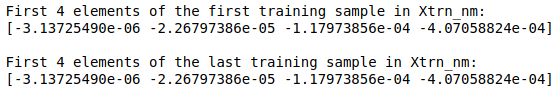
\includegraphics[width=1\textwidth]{images/q11.png}
      \end{answerbox}
  


   \end{subquestion}
   %
   % ==============================
   % 
   % Q1.2
   \begin{subquestion}{(4 points)
      Using {\tt Xtrn} and Euclidean distance
      measure, for each class,
      find the two closest samples and two furthest
      samples of that class to the mean vector of the class.
    }  \label{Q1.2}




  \begin{answerbox}{52em}
    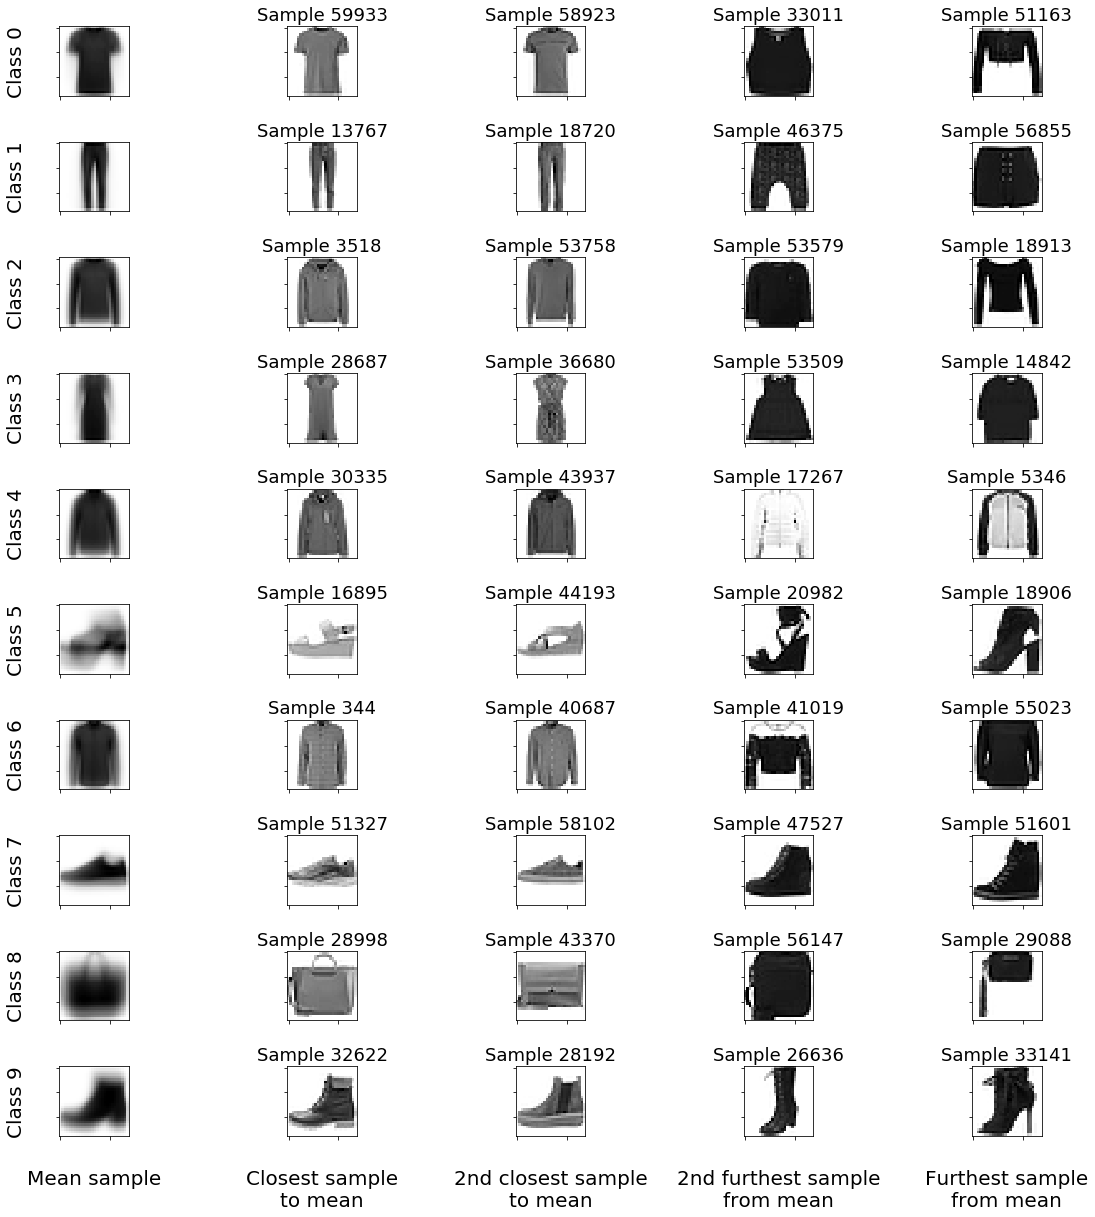
\includegraphics[width=1\textwidth]{images/q12.png}
    Explain your findings briefly...
  \end{answerbox}



   \end{subquestion}

   % 
   % Q1.3
   \begin{subquestion}{(3 points)
       Apply Principal Component Analysis (PCA) to the data of {\tt
         Xtrn\_nm} using \href{https://scikit-learn.org/0.19/modules/generated/sklearn.decomposition.PCA.html}{sklearn.decomposition.PCA}, and report the variances of projected data for the first five principal components in a table.
        Note that you should use {\tt Xtrn\_nm} instead of {\tt Xtrn}.
     } \label{Q1.pca.variance}



    \begin{answerbox}{15em}
        \begin{center}
        \textbf{\large{\underline{Calculating the variances of the projected data in Xtrn\_nm}}}\\
        \textbf{\large{\underline{for the first five principal components}}}\\
        \vspace{0.5cm}
        \begin{tabular}{ |c|c| } \hline
        \textbf{Principal Component \#} & \textbf{Explained Variance} \\ \hline
        1 & 19.81 \\
        2 & 12.112 \\
        3 & 4.106 \\
        4 & 3.382 \\
        5 & 2.625 \\\hline
        \end{tabular}
        \end{center}
    \end{answerbox}
    


   \end{subquestion}

   %==============================
   % Q1.4
   \begin{subquestion}{(3 points)
       Plot a graph of the cumulative explained variance ratio as a function of the number of principal components, $K$, where $1\le K \le 784$.
       Discuss the result briefly.
     } \label{Q1.plot.pca.variance}
   

      \begin{answerbox}{50em}
         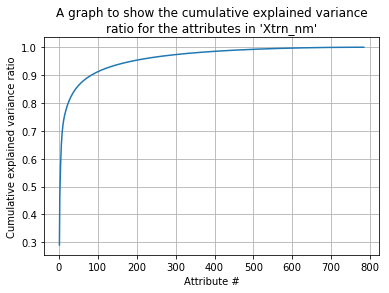
\includegraphics[width=1\textwidth]{images/q14.png}
        Discuss the result briefly...
      \end{answerbox}
  


   \end{subquestion}

   %==============================
   % Q1.5
   \begin{subquestion}{(4 points)
      Display the images of the first 10 principal components in
      a 2-by-5 grid, putting the image of 1st principal component on
      the top left corner, followed by the one of 2nd component to the right.
      Discuss your findings briefly.
     } \label{Q1.disp.pca}
   

      \begin{answerbox}{35em}
         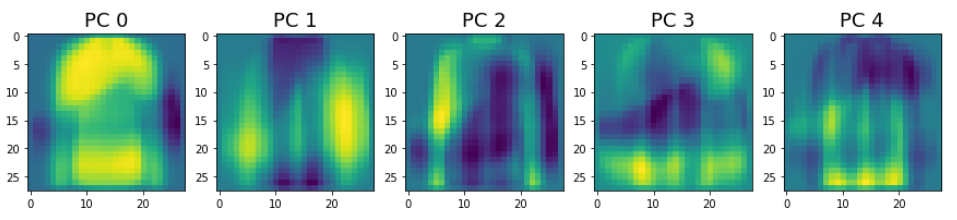
\includegraphics[width=1\textwidth]{images/q151.png}
         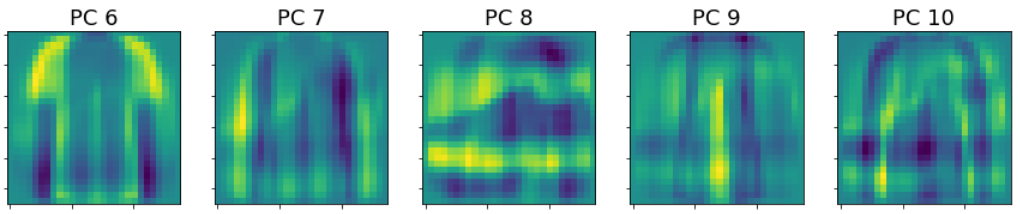
\includegraphics[width=1\textwidth]{images/q152.png}
        Discuss your findings briefly...\\
        We must note that these images are not distinct given they were calculated using the normalized dataset
      \end{answerbox}
  


   \end{subquestion}

   %==============================
   % Q1.6
   \begin{subquestion}{(5 points)
       Using \texttt{Xtrn\_nm}, 
       for each class and for each number of principal components $K =
       5, 20, 50, 200$, apply dimensionality reduction with PCA to the
       first sample in the class, reconstruct the sample from the
       dimensionality-reduced sample, and 
       report the Root Mean Square Error (RMSE) between the
       original sample in {\tt Xtrn\_nm} and reconstructed one.
     } \label{Q1.6}

     

      \begin{answerbox}{28em}
        \begin{center}
        \large{\textbf{A table to show the RMSE between the original and the}}\\
        \large{\textbf{reconstructed version of the first sample for every}}\\
        \large{\textbf{class with varying numbers of PCA components (K)}} \\
        \vspace{0.3cm}
        \normalsize{*Each class sample is reconstructed by reducing the sample to K dimensions and then is transformed back to the original number of dimensions, this is all done via the sklearn PCA implementation.}\\
        \vspace{0.5cm}
        \begin{tabular}{ |c|c|c|c|c|c| } \hline
            \textbf{RMSE} & K = 5 & K = 20 & K = 50 & K = 200 \\ \hline
            Class = 0 & 0.256 & 0.15 & 0.128 & 0.063 \\
            Class = 1 & 0.198 & 0.14 & 0.095 & 0.037 \\
            Class = 2 & 0.199 & 0.146 & 0.124 & 0.08 \\
            Class = 3 & 0.146 & 0.107 & 0.083 & 0.056 \\
            Class = 4 & 0.118 & 0.103 & 0.088 & 0.045 \\
            Class = 5 & 0.181 & 0.159 & 0.142 & 0.09 \\
            Class = 6 & 0.129 & 0.096 & 0.072 & 0.045 \\
            Class = 7 & 0.166 & 0.128 & 0.106 & 0.063 \\
            Class = 8 & 0.223 & 0.145 & 0.124 & 0.094 \\
            Class = 9 & 0.184 & 0.151 & 0.122 & 0.072 \\
            \hline
        \end{tabular}
        \end{center}
      \end{answerbox}
  


   \end{subquestion}
   
   %==============================
   % Q1.7
   \begin{subquestion}{(4 points)
       Display the image for each of the reconstructed samples in
       a 10-by-4 grid, where each row corresponds to a class and
       each row column corresponds to a value of $K=5, \; 20, \; 50, \; 200$.
     } \label{Q1.7}


   

      \begin{answerbox}{52em}
         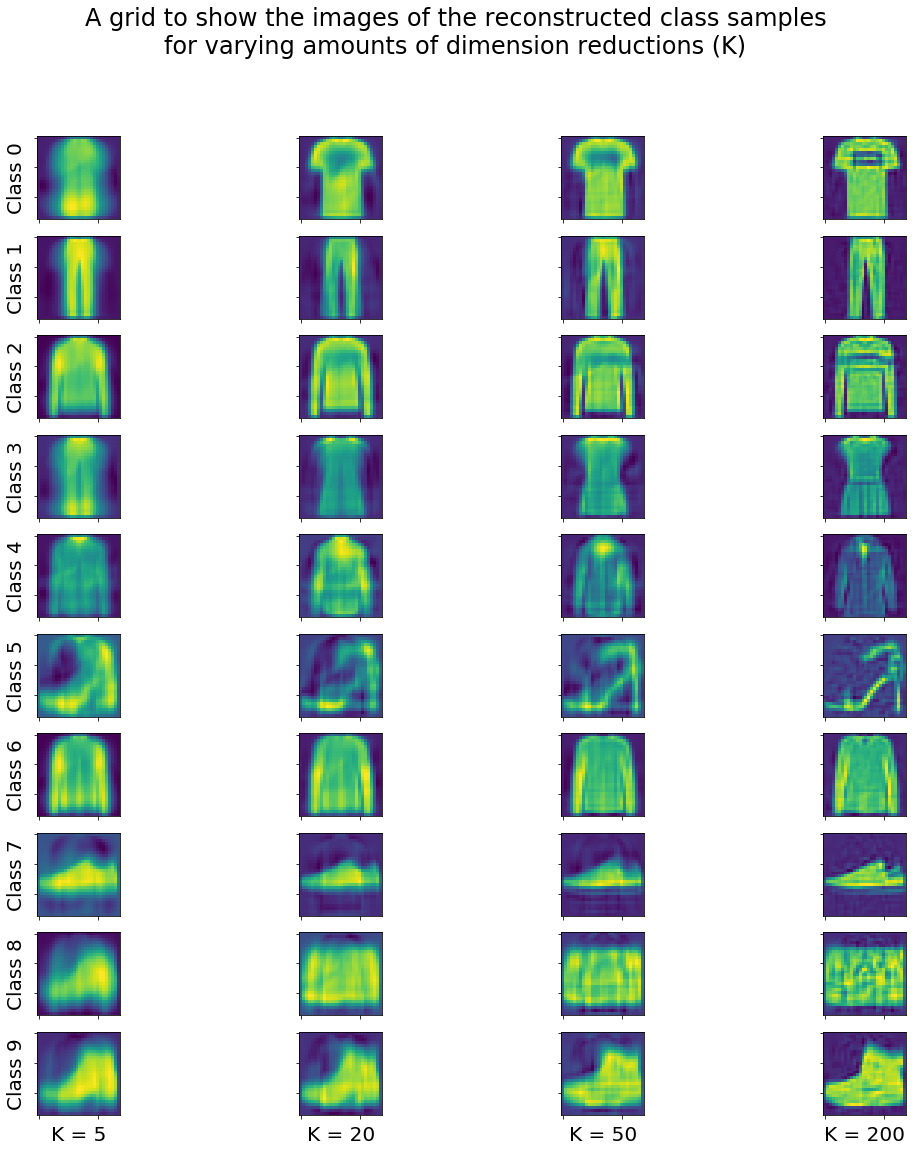
\includegraphics[width=1\textwidth]{images/q17.png}
        Discuss your findings briefly...
      \end{answerbox}
  


   \end{subquestion}
   %==============================
   %
   %==============================
   % Q1.8
   \begin{subquestion}{(4 points)
       Plot all the test samples (\texttt{Xtrn\_nm}) on the
       two-dimensional PCA plane you obtained in \refQ{Q1.pca.variance}, where each sample is
       represented as a small point with a colour specific to the class of
       the sample.  Use the 'coolwarm' colormap for plotting.
     } \label{Q1.8}


   

      \begin{answerbox}{40em}
         Your Answer Here
      \end{answerbox}
  


   \end{subquestion}
   %
   %==============================
   

\end{question}
%%%%%%%%%%%%%%%%%%%%%%%%%%%%%%%%%%%%%%%%%%%%%%%%%%%%%%%%%%%%%%%%%%%%%%%%%%%%%%
%============================================================================%
%%%%%%%%%%%%%%%%%%%%%%%%%%%%%%%%%%%%%%%%%%%%%%%%%%%%%%%%%%%%%%%%%%%%%%%%%%%%%%
\clearpage
%
% Question 2
%
\begin{question}{(25 total points) Logistic regression and SVM}

  \questiontext{In this question we will explore 
    classification of image data with logistic regression and support
    vector machines (SVM) and visualisation 
    of decision regions.
  }
  


  \medskip
   %==============================
   % Q2.1
   \begin{subquestion}{(3 points)
       Carry out a classification experiment with
       \href{https://scikit-learn.org/0.19/modules/generated/sklearn.linear\_model.LogisticRegression.html}{multinomial logistic regression},
       and report the classification accuracy and confusion matrix (in
       numbers rather than in graphical representation such as heatmap)
       for the test set.
     } \label{Q2.1}


   

      \begin{answerbox}{37em}
         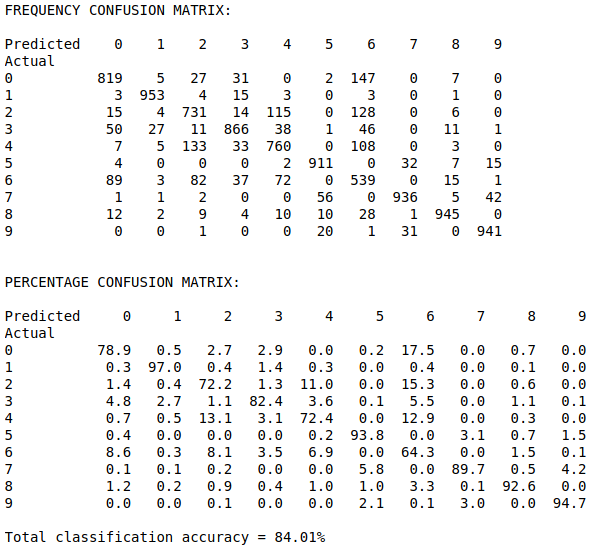
\includegraphics[width=1\textwidth]{images/q21.png}
      \end{answerbox}
  


   \end{subquestion}
   %
   % ==============================
   %
   %==============================
   % Q2.2
   \begin{subquestion}{(3 points)
       Carry out a classification experiment with
       \href{https://scikit-learn.org/0.19/modules/generated/sklearn.svm.SVC.html}{SVM classifiers}, and report the
       mean accuracy and confusion matrix (in numbers) for the test
       set.
     } \label{Q2.2}


   

      \begin{answerbox}{37em}
         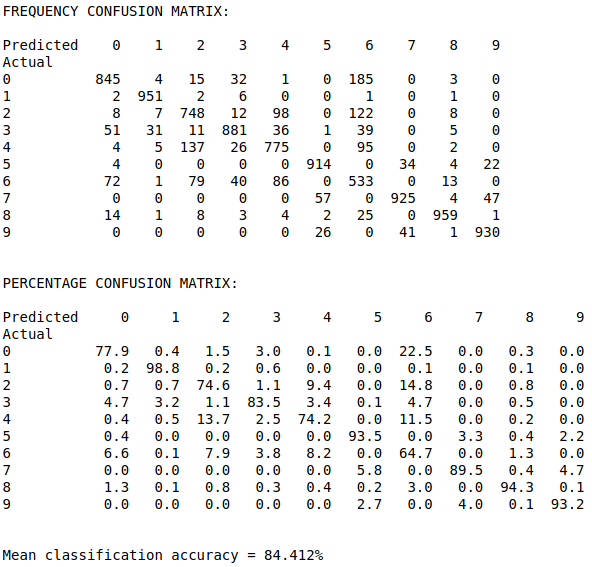
\includegraphics[width=1\textwidth]{images/q22.png}
      \end{answerbox}
  


   \end{subquestion}
   %
   % ==============================
   %
   %==============================
   % Q2.3
   \begin{subquestion}{(6 points)
       We now want to visualise the decision regions for the logistic
       regression classifier we trained in \refQ{Q2.1}.
     } \label{Q2.3}


   

      \begin{answerbox}{35em}
         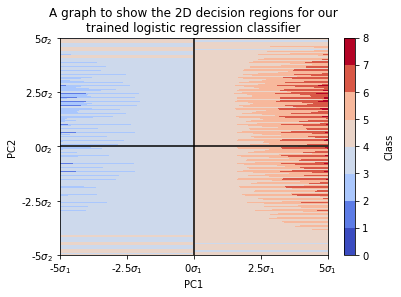
\includegraphics[width=1\textwidth]{images/q23.png}
      \end{answerbox}
  


   \end{subquestion}
   %
   % ==============================
   %
   %==============================
   % Q2.4
   \begin{subquestion}{(4 points)
       Using the same method as the one above, plot the decision regions for
       the SVM classifier you trained in \refQ{Q2.2}.
       Comparing the result with that you obtained in \refQ{Q2.3}, discuss your
       findings briefly.
     } \label{Q2.4}
   

      \begin{answerbox}{35em}
         Your Answer Here
      \end{answerbox}
  


   \end{subquestion}
   %
   % ==============================
   %

   %==============================
   % Q2.5
   \begin{subquestion}{(6 points)
       We used default parameters for the SVM in \refQ{Q2.2}.
       We now want to tune the parameters by using cross-validation.
       To reduce the time for experiments, you pick up the first 1000
       training samples from each class to create \texttt{Xsmall}, so that \texttt{Xsmall}
       contains 10,000 samples in total. Accordingly, you create
       labels, \texttt{Ysmall}.
     } \label{Q2.5}


   

      \begin{answerbox}{34em}
        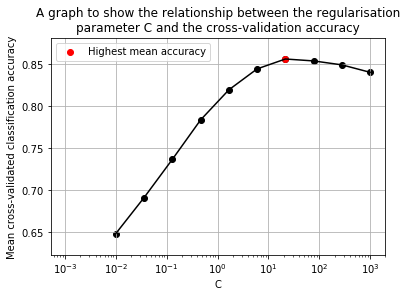
\includegraphics[width=1\textwidth]{images/q25.png}
        \\
        \\
        \textbf{\underline{Optimal accuracy achieved and it's respective value of C:}} \\
        \\
        $Accuracy \approx 85.65 \%$  where  $C \approx 10^{1.33}$
      \end{answerbox}
  


   \end{subquestion}
   %
   % ==============================
   %
   %==============================
   % Q2.6
   \begin{subquestion}{(3 points)
       Train the SVM classifier on the whole training set by using the
       optimal value of $C$ you found in \refQ{Q2.5}. 
     } \label{Q2.6}


       

      \begin{answerbox}{10em}
        \large{\textbf{\underline{Classification accuracy of our trained SVM using $\mathbf{C = 10^{\frac{4}{3}}}$}}}\\
        \\
        \normalsize{
        Training accuracy $\approx 86.768\%$\\
        Testing accuracy $\approx 85.02\%$
        }
      \end{answerbox}
  


   \end{subquestion}
   %
   % ==============================
   %
%
%

\end{question}
%%%%%%%%%%%%%%%%%%%%%%%%%%%%%%%%%%%%%%%%%%%%%%%%%%%%%%%%%%%%%%%%%%%%%%%%%%%%%%
%============================================================================%
%%%%%%%%%%%%%%%%%%%%%%%%%%%%%%%%%%%%%%%%%%%%%%%%%%%%%%%%%%%%%%%%%%%%%%%%%%%%%%
\clearpage
%
% Question 3
%

\begin{question}{(20 total points) Clustering and Gaussian Mixture Models}  


  \questiontext{In this question we will explore K-means clustering,
    hierarchical clustering, and GMMs.
  }
  


  \medskip
   %==============================
   % Q3.1
   \begin{subquestion}{(3 points)
       Apply k-means clustering on {\tt Xtrn} for $k = 22$, where we use
       \href{https://scikit-learn.org/0.19/modules/generated/sklearn.cluster.KMeans.html}{sklearn.cluster.KMeans}
       with the parameters {\tt n\_clusters=22} and {\tt random\_state=1}.
       Report the sum of squared distances of samples to their closest
       cluster centre, and the number of samples for each cluster.
     } \label{Q3.1}
   

      \begin{answerbox}{35em}
         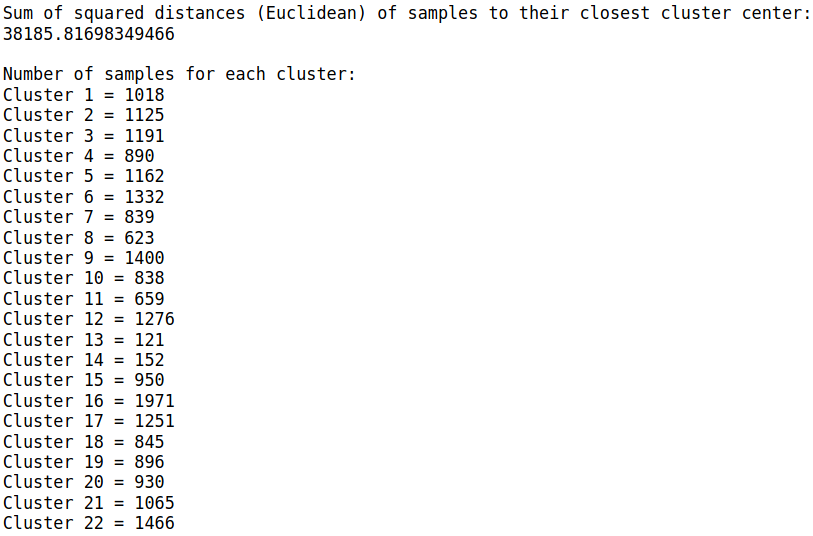
\includegraphics[width=1\textwidth]{images/q31.png}
      \end{answerbox}
  


   \end{subquestion}
   %
   % ==============================
   %
   %==============================
   % Q3.2
   \begin{subquestion}{(3 points)
       Using the training set only,
       calculate the mean vector for each language, and plot the mean
       vectors of all the 22 languages on a 2D-PCA plane, where you
       apply PCA on the set of 22 mean vectors without applying
       standardisation.  
       On the same figure, plot the cluster centres obtained in \refQ{Q3.1}.
     } \label{Q3.2}

   

      \begin{answerbox}{53em}
         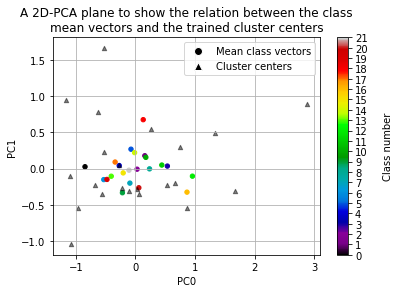
\includegraphics[width=1\textwidth]{images/q32.png}
      \end{answerbox}
  


   \end{subquestion}
   %
   % ==============================
   %
   %==============================
   % Q3.3
   \begin{subquestion}{(3 points)
       We now apply hierarchical clustering on the training data set
       to see if there are any structures in the spoken languages.
     } \label{Q3.3}


     

      \begin{answerbox}{40em}
        \textbf{\large{\underline{A dendogram to show the hierarchical clustering of the mean}}}\\
        \textbf{\large{\underline{vectors for each language}}}\\
        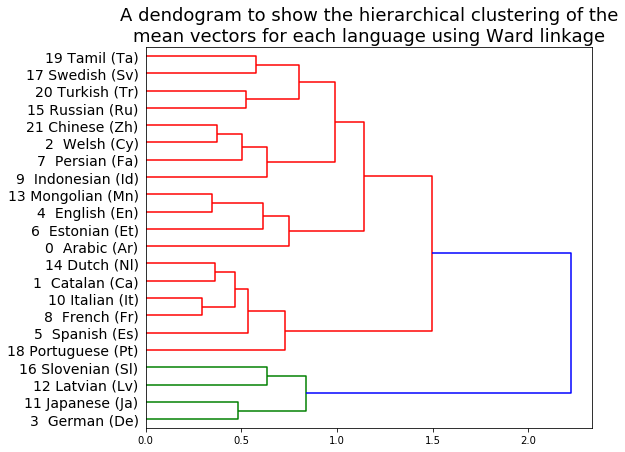
\includegraphics[width=1\textwidth]{images/q33.png}
        \\
        \\
        This dendogram illustrates how each cluster from our dataset is composed and thus ultimately represents the hierarchy of similarities between the classes in our data.\\
        \\
        From this we can deduce that Italian and French have the most similar mean vectors and thereby are the most "similar" languages. In contrast we can see that Latvian has the most dissimilar mean vector from all other languages and thereby is the most "unique" language.
      \end{answerbox}
  


   \end{subquestion}
   %
   % ==============================
   %
   %==============================
   % Q3.4
   \begin{subquestion}{(5 points)
       We here extend the hierarchical clustering done in \refQ{Q3.3} by
       using multiple samples from each language.
     } \label{Q3.4}


   

      \begin{answerbox}{55em}
        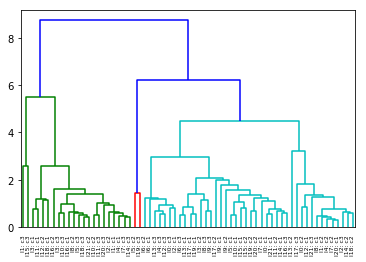
\includegraphics[width=0.65\textwidth]{images/q34ward.png}
        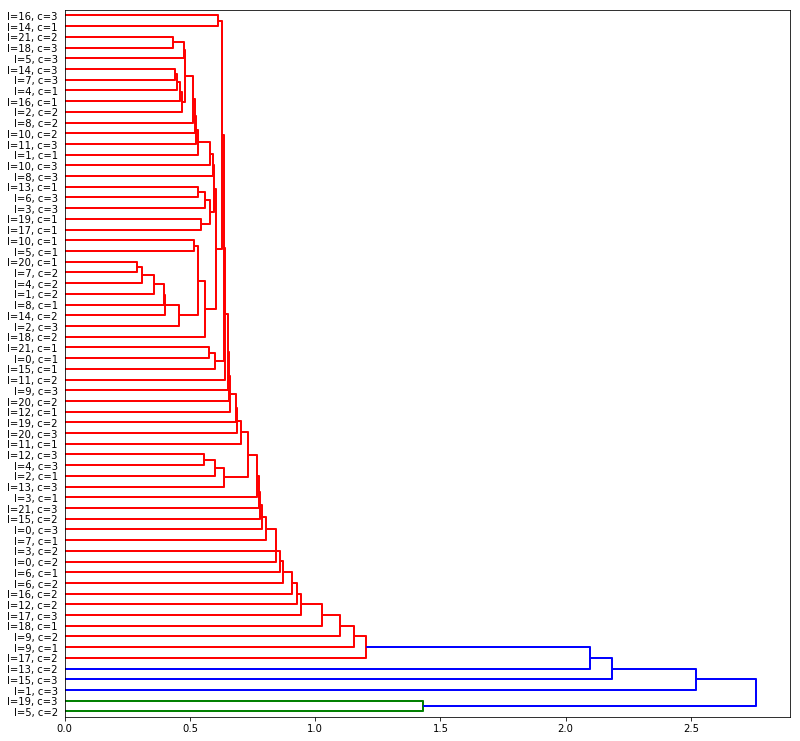
\includegraphics[width=0.65\textwidth]{images/q34single.png}
        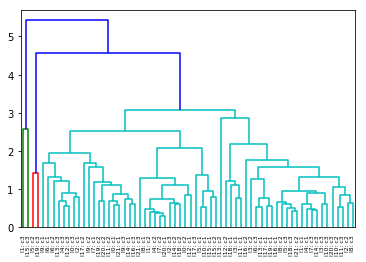
\includegraphics[width=0.65\textwidth]{images/q34complete.png} 
      \end{answerbox}
  


   \end{subquestion}
   %
   % ==============================
   %
   %==============================
   % Q3.5
   \begin{subquestion}{(6 points)
       We now consider Gaussian mixture model (GMM), whose
       probability distribution function (pdf) is given as
       a linear combination of Gaussian or normal distributions, i.e.,
     } \label{Q3.5}




      \begin{answerbox}{30em}
         Your Answer Here
      \end{answerbox}
  


   \end{subquestion}
   %
   %==============================

   % ==============================
   
\end{question}
\end{document}
